\subsection{Captura 2 - Starbucks}

Esta captura se realizó en el Starbucks de Avenida Cabildo y Juramento alrededor de las cuatro de la tarde \textit{(con mucha gente)} durante veinticinco minutos, logrando capturar $19829$ paquetes de los cuales $1196$ son paquetes ARP.

\begin{figure}[H]
  \centering
    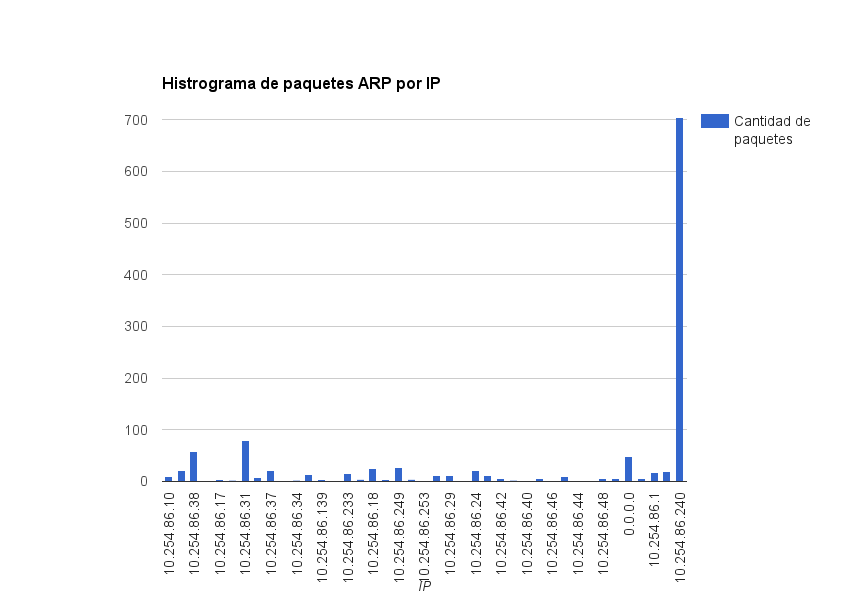
\includegraphics[width=1.1\textwidth]{imagenes/starbucks/histograma.png}
  \caption{Histograma de los símbolos de la fuente $S_1$}
  \label{fig:ejemplo}
\end{figure}

En esta red aparece la IP \textit{0.0.0.0}. No apareció en la anterior captura y nos llamó la atención su particular forma. Investigamos 
acerca de su semántica y encontramos que se le dan varios usos. Entre ellos los más comunes son:
\begin{itemize}
  \item Los host suelen mostrar que tienen una IP 0.0.0.0 cuando no cuentan con una conexión TCP/IP disponible. Es decir, utilizan esta IP para comunicarse con un servidor \textit{DHCP}, el cual les proveerá una IP valida.
  \item Las aplicaciones TCP/IP usan la dirección 0.0.0.0 para poder monitorizar el tráfico de cualquier dirección IP válida.
  \item Los mensajes IP contienen la dirección 0.0.0.0 en sus headers cuando la fuente del mensaje es desconocida.
\end{itemize}
Creemos que el único caso que tiene sentido que aparezca en una captura es el primero.

\begin{figure}[H]
  \centering
    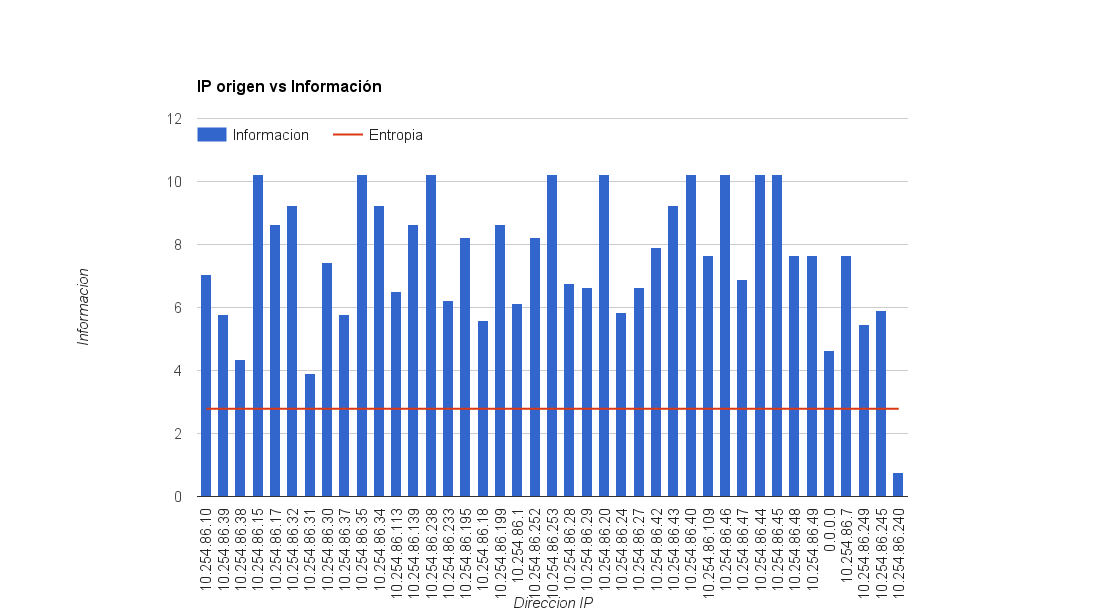
\includegraphics[width=1.1\textwidth]{imagenes/starbucks/ip_informacion.png}
  \caption{Información de los símbolos de la fuente $S_1$}
  \label{fig:ejemplo}
\end{figure}

Nuevamente podemos apreciar la correlación entre este gráfico y el anterior, aunque entre éstos no sea tan clara. El nodo distinguido, aquel que cuenta con la mayor frecuencia y la información
por debajo de la entropía, debe ser el router.

\begin{figure}[H]
  \centering
    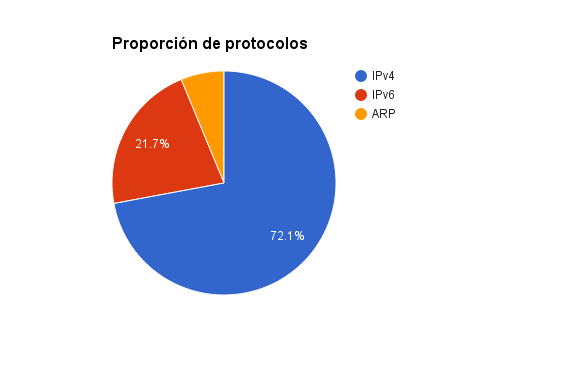
\includegraphics[width=0.7\textwidth]{imagenes/starbucks/proporcion_protocolos.png}
  \caption{Proporción de protocolos observados en el trafico de la red Starbucks}
  \label{fig:ejemplo}
\end{figure}

Se puede ver que en esta red, a diferencia de la anterior, el uso del protocolo \textit{IPv6} es mucho mas frecuente, aunque el protocolo \textit{IPv4} sigue siendo el predominante. 
También podemos ver que el overhead impuesto por ARP es del 6.1\% del tráfico de la red. Creemos que una posible causa por la cual el overhead se haya duplicado con respecto al 
encontrado en la red S.I.S.A es que la red es pública, por lo tanto, los dispositivos que la utilizan se renuevan constantemente imponiendo sobre el router una mayor carga de resolución
de direcciones.

\begin{figure}[H]
  \centering
    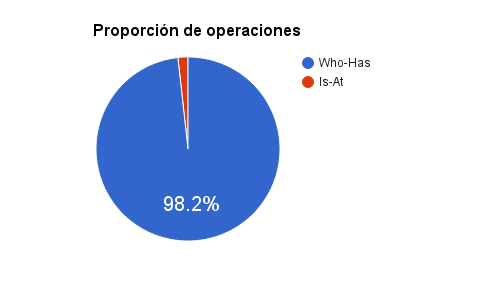
\includegraphics[width=0.9\textwidth]{imagenes/starbucks/proporcion_paquetes_arp.png}
  \caption{Proporción de paquetes who-has vs is-at en red Starbucks}
  \label{fig:ejemplo}
\end{figure}

Al igual que sucedió en la captura anterior, los paquetes \textit{who-has} predominan en esta red. Creemos que los motivos son los mismos que en la captura anterior.

\begin{figure}[H]
  \centering
    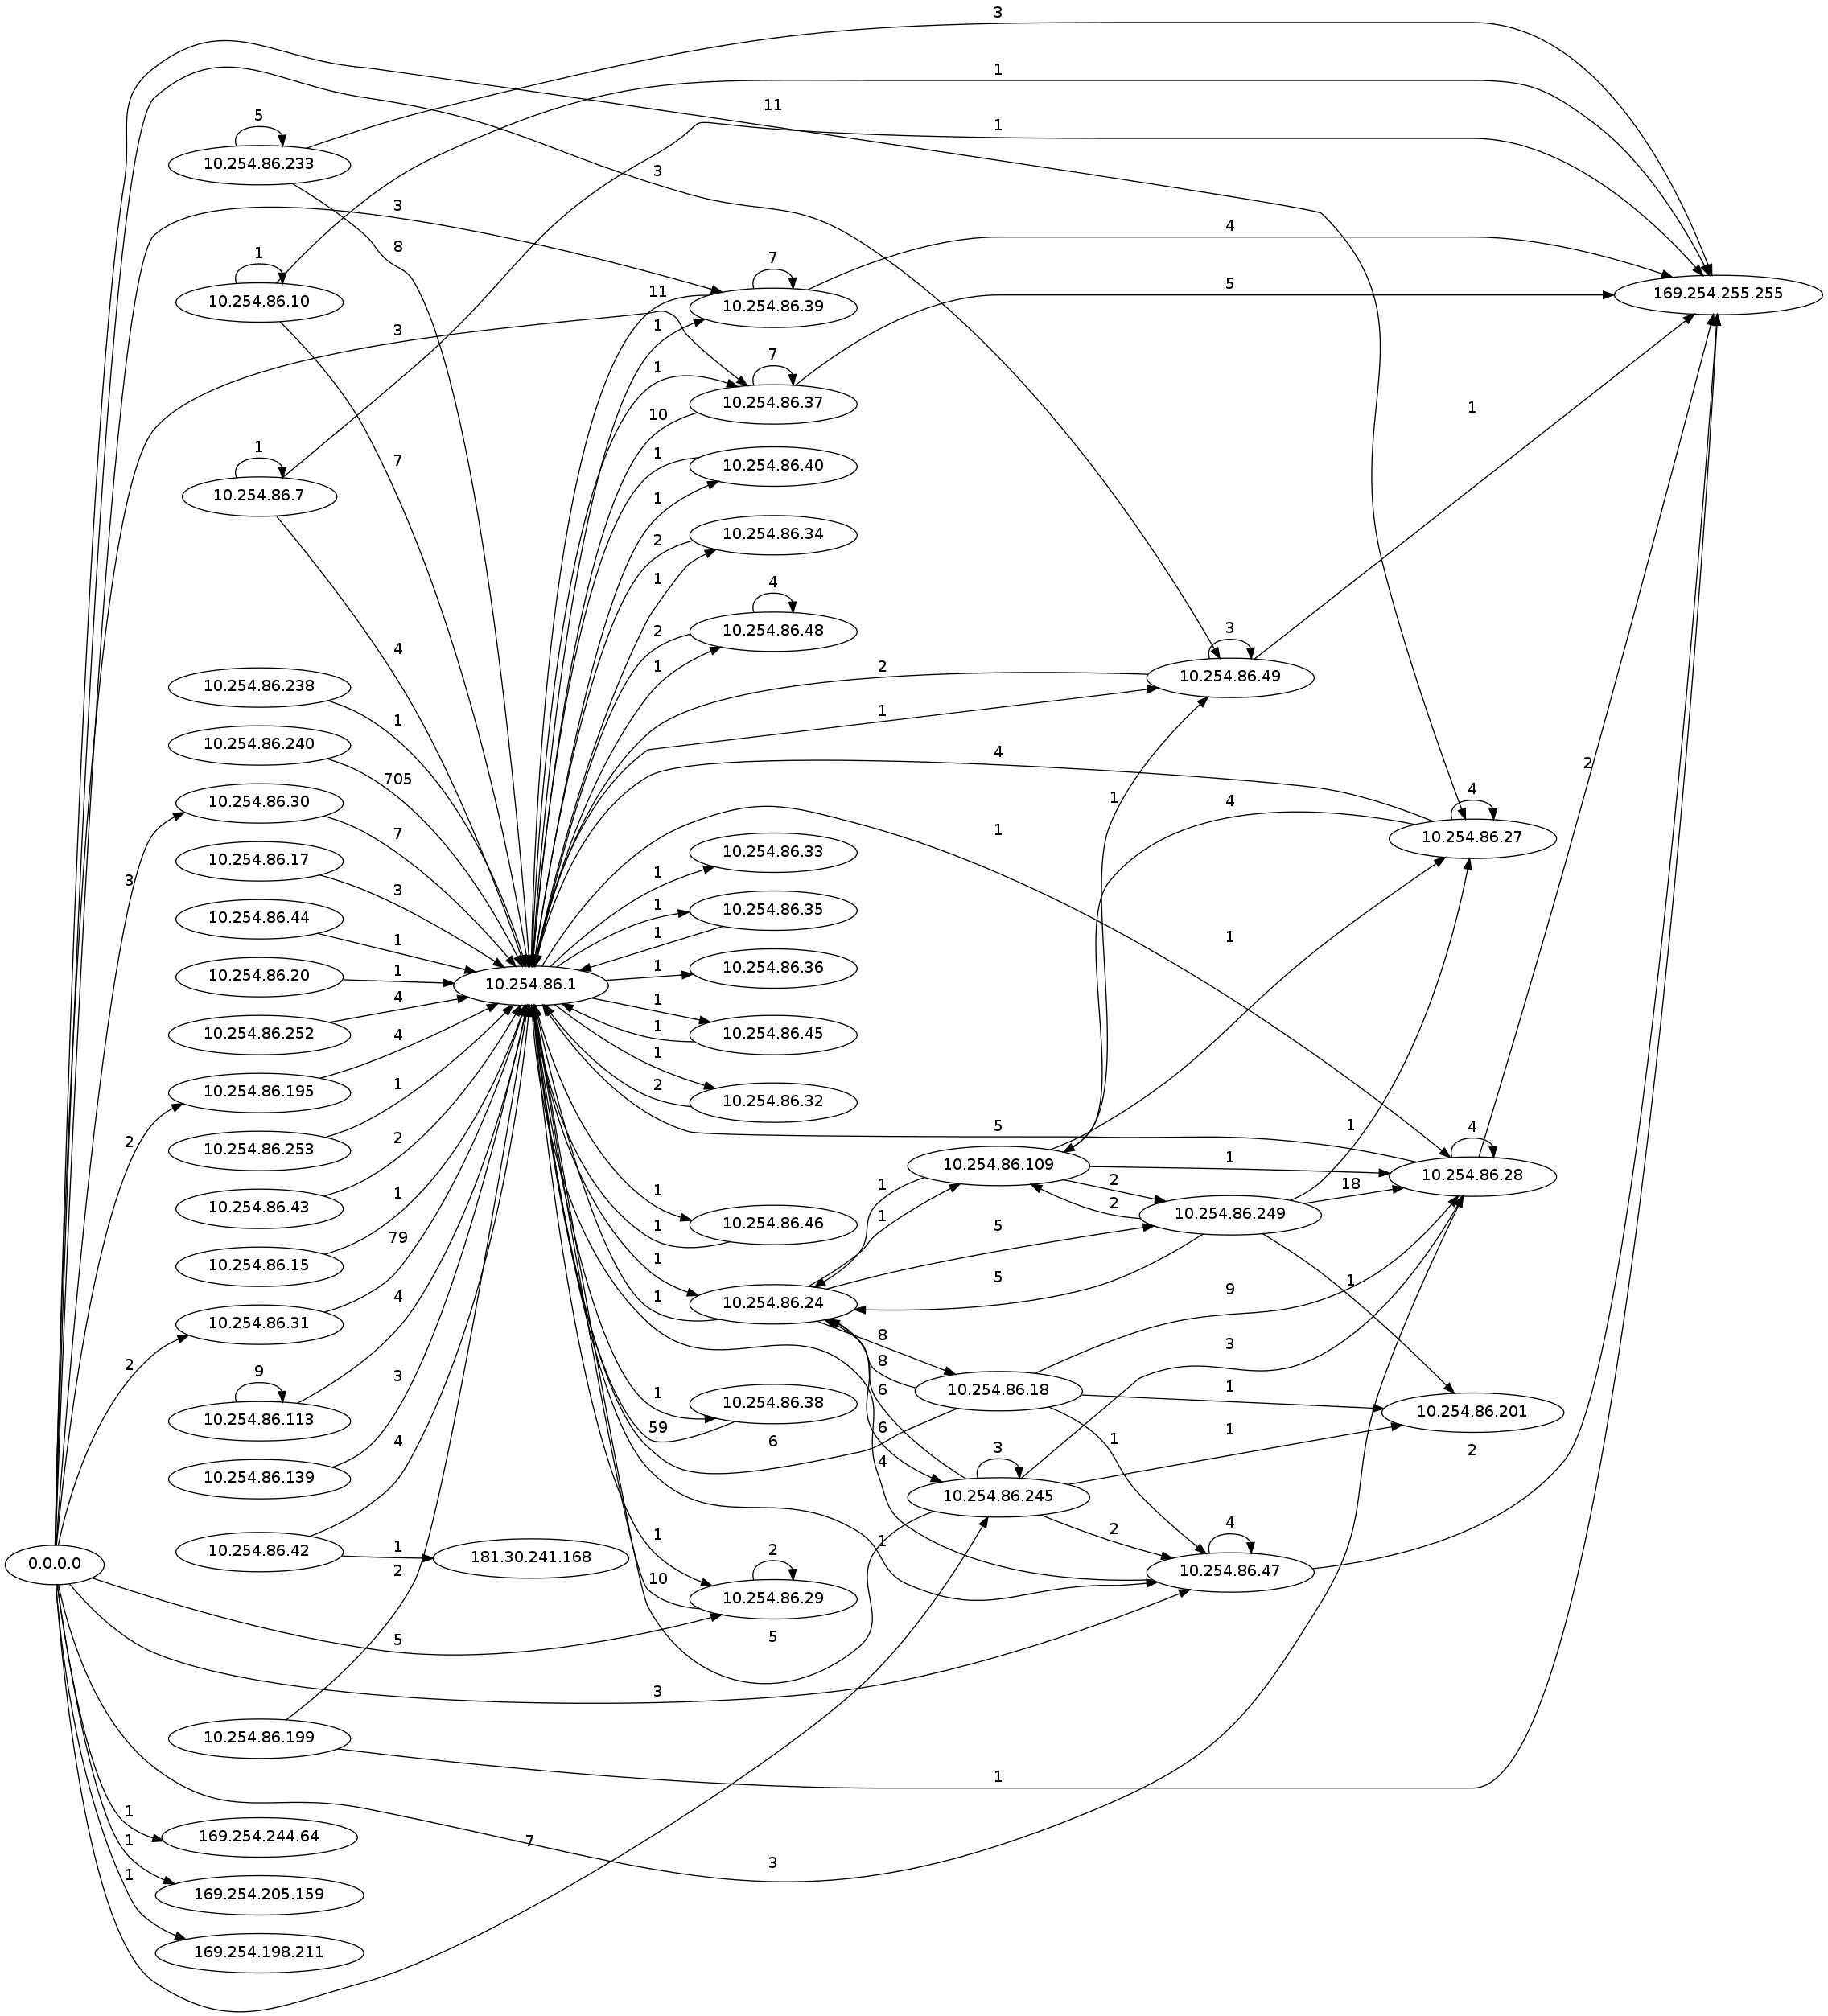
\includegraphics[width=1.2\textwidth]{imagenes/starbucks/digrafo_starbucks.png}
  \caption{Trafico de paquetes ARP entre las IP de la red Starbucks}
  \label{fig:ejemplo}
\end{figure}


\begin{figure}[H]
  \centering
    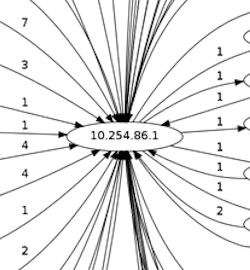
\includegraphics[width=0.4\textwidth]{imagenes/starbucks/router.png}
  \caption{Direccion IP del router de la red de Starbucks}
  \label{fig:ejemplo}
\end{figure}

Claramente la dirección IP 10.254.86.1 concentra todo el trafico ARP de la red y, por lo tanto, podemos presumir que esta es la dirección IP del router.

\begin{figure}[H]
  \centering
    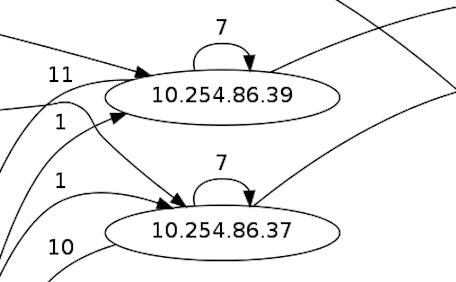
\includegraphics[width=0.4\textwidth]{imagenes/starbucks/loop.png}
  \caption{Un host enviándose paquetes ARP a si mismo}
  \label{fig:ejemplo}
\end{figure}

Esta situación, en donde un host se envía paquetes ARP a si mismo \textit{(misma IP de origen y de destino)} sucede en muchas ocasiones. Se trata de una forma de uso del protocolo llamada \textit{Gratuitous ARP}\footnote{Gratuitous ARP: \url{http://wiki.wireshark.org/Gratuitous_ARP}} que se utiliza, mayormente, para detectar conflictos de IP en la red o para actualizar la información en las tablas de los otros host de la red. En resumen, cuando un host envía paquete de este estilo espera no recibir ninguna respuesta, ya que si la recibiera significaría que hay otro host en la red que tiene asignada su misma dirección IP.

\begin{figure}[H]
  \centering
    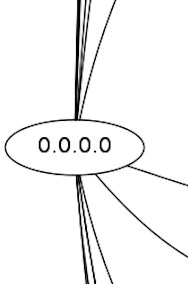
\includegraphics[width=0.23\textwidth]{imagenes/starbucks/cerocero.png}
  \caption{Paquetes ARP son enviados desde la dirección IP 0.0.0.0}
  \label{fig:ejemplo}
\end{figure}

En esta red pudimos detectar muchos paquetes \textit{who-has} con 0.0.0.0 como dirección IP origen. Además, la red cuenta con un servidor DHCP y en esos casos tiene una semántica especial. 
Esta IP es utilizada por los host de una red que cuenta con un servidor DHCP durante el tiempo que le toma al host elegir una IP de entre las IPs ofrecidas (\textit{libres}) por el servidor DHCP. Durante este proceso el host utiliza la IP 0.0.0.0 como origen y la IP que eligió (\textit{de entre las que el servidor DHCP le ofreció}) como destino para hacer broadcast de un paquete ARP \textit{who-has} en la red para asegurarse de que ningún host en la red responde el mensaje, es decir, que la IP que eligió este efectivamente libre.


\begin{figure}[H]
  \centering
    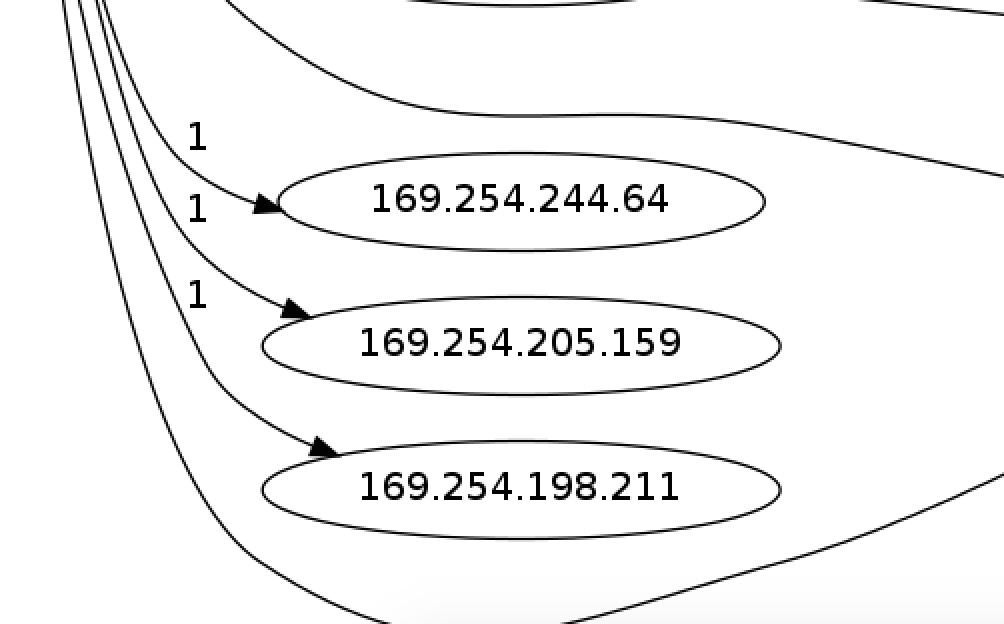
\includegraphics[width=0.4\textwidth]{imagenes/starbucks/unoNueve.png}
  \caption{IPs en el rango 169.254.0.0/16}
  \label{fig:ejemplo}
\end{figure}

Las direcciones IP en el rango 169.254.0.0/16 son \textit{direcciones de enlace local}\footnote{Fuente: \url{http://es.wikipedia.org/wiki/Direcci\%C3\%B3n\_de\_Enlace-Local}}, y son direcciones reservadas unicamente para comunicacion dentro de una subred local. En IPv4, las direcciones de enlace local pueden usarse cuando no hay disponible un mecanismo externo de configuración de direcciones, tal como DHCP, u otro mecanismo principal de configuración ha fallado. En IPv6 \textit{(el cual recordemos que ocupa mas de un 20\% del trafico de esta red)}, las direcciones de enlace local son necesarias para el funcionamiento interno de varios componentes del protocolo.

\newpage
